\documentclass{standalone}
\usepackage{tikz}
\usetikzlibrary{shapes.geometric, arrows}

\definecolor{mycolor}{RGB}{0, 153, 255}
\tikzstyle{process} = [rectangle, rounded corners,
                       minimum width=2cm, minimum height=1cm,
                       text centered, draw=black, fill=mycolor,
                       text=white, line width=0.3mm]

\tikzstyle{arrow} = [thick,->,>=stealth]

\begin{document}
    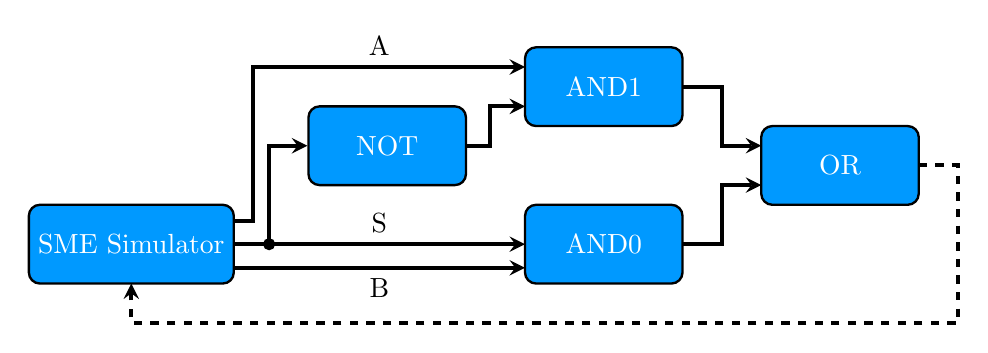
\begin{tikzpicture}[node distance=2cm]
        
        \node (Simulator) [process] {SME Simulator};
        
        %NOT Gates
        \node (NOT) [process, right of = Simulator, xshift=1.25cm, yshift=1.25cm] {NOT};
        
        %Simulator to NOT gate
        \draw [arrow, line width=0.5mm] (1.75, 0) |-  (NOT);
        \filldraw[black] (1.75, 0) circle (2pt);
        
        %AND Gates
        \node (AND0) [process, right of = NOT, xshift=0.75cm, yshift=-1.25cm] {AND0};
        \node (AND1) [process, above of = AND0, xshift=0cm] {AND1};
        %OR Gate
        \node (OR) [process, right of = AND0, xshift=1cm, yshift=1cm] {OR};
        
        %Lines to AND1 gate
        \draw [arrow, line width=0.5mm] (1.3, 0.3) -- ++(0.25,0) |- node [above,xshift=1.6cm] {A} (5, 2.25);
        \draw [arrow, line width=0.5mm] (NOT) -- ++(1.3,0) |-  (5, 1.75);

        %Lines to AND0 gate
        \draw [arrow, line width=0.5mm] (1.3,0) -- node [above] {S} (5,0);
        \draw [arrow, line width=0.5mm] (1.3,-0.3) -- node [below] {B} (5,-0.3);
        
        %Lines to Or gate
        \draw [arrow, line width=0.5mm] (7,0) -- ++(0.5,0) |- (8,0.75);
        \draw [arrow, line width=0.5mm] (7,2) -- ++(0.5, 0)  |- (8,1.25);
        
        %Output line to simulator
        %AND3
        \draw [arrow, line width=0.5mm, dashed] (10,1) -- ++(0.5, 0) -- ++(0,-2) -- ++(-10.5,0) -- (0,-0.5);
        
    
    \end{tikzpicture}
\end{document}
